\chapter{}
Quando o sítio entrou na nossa vida, as tias já estavam mais velhas, os primos já haviam se casado e constituído família e reunir o clã dos Filpi se tornou mais difícil.
As tias tiveram que se dividir por ocasião das festas e feriados, entre a fazenda do Tio Totó e o sítio do mano Mathias.
Acabaram-se os Natais na casa delas e começamos a fazer nossas próprias festas.
Era erguer o mastro, fazer fogueira e enfeitar o terreiro com arcos de bambu e bandeirolas em junho, que as festas juninas eram as de que meu pai mais gostava; espalhar capim e cenouras meio roídas pela casa na Páscoa, para ver as crianças seguirem os vestígios do Coelho, ansiosas para achar os ovos escondidos e, em dezembro, preparar o presépio na capela, enfeitar o pinheiro, encomendar o cabrito da ``pastorale'', o tradicional ensopado cuja receita fora trazida pelos mais velhos de Novi Veglia e que há séculos reinava na mesa dos Filpi nas grandes ocasiões.
Havia também os ``canarícoli'', doces particularmente brutos, que minha bisavó materna, Lectizia Grecco Credidio, aprendeu a fazer com a gente de Catanzaro e que acabaram sendo adotados por toda a família.
Tia Odila, caçoando, chamava-os de ``os bombons de vovó'' antes de enunciar a mimosa receita: cinco quilos de farinha, três litros de óleo, igual medida de vinho, mais outro tanto de mel, duas ou três ``mãos'' de especiarias moídas (cravo, canela e noz-moscada) e por aí afora.


A confecção dos canarícoli era por si só uma festa.
Era preciso reservar um dia todo para a empreitada.
A massa que resultava da mistura dos ingredientes era de tal forma pesada que só os braços robustos da Tia Glória conseguiam a façanha de sová-la adequadamente.
Ainda assim, ela passava a semana seguinte se queixando de dores.
Posta a fermentar, a massa crescida era dividida entre meia dúzia de mulheres reunidas em torno de uma mesa grande na qual aquela enormidade era modelada em longos cordões roliços de polegada e meia de diâmetro.
Uma ou duas recrutas, geralmente nós, as sobrinhas, íamos cortando os cordões em roletes iguais de cinco ou seis centímetros de comprimento, passando-os em seguida num comprido ralador para frisá-los, de modo a assegurar a aderência do mel em que seriam banhados no final.
A etapa seguinte era a mais sacrificada e a mais importante: a fritura.
Um grande tacho de óleo era posto a ferver sobre o fogão de lenha até atingir uma temperatura vulcânica.
Suando em bicas, as tias iam se revezando no serviço de dourar os bolinhos até deixá-los da cor de madeira envernizada, todos por igual.
Aí, era só recolhê-los com a escumadeira e deixá-los escorrendo na peneira forrada com papel de embrulhar pão.
Ao fim do dia, os doces eram encerrados em grandes latas de alumínio repletas de mel, de onde só seriam libertados na véspera do Natal.
Ficava, para assanhar a gula da criançada, apenas aquele aroma intenso de especiarias a pairar pelo ambiente por mais dois ou três dias, pelo menos.

Outro momento importante nos Natais do sítio era o de decidir quem seria o Papai Noel da vez.
Por muito tempo a escolha recaiu sobre o Renato por causa do seu físico avantajado.
Mas, coitado, nunca, em todos os anos que lhe coube encarnar o bom velhinho, conseguimos encontrar bota que servisse nos seus gordos pés número quarenta e quatro.
As crianças achavam que era por cansaço que o pobre Noel erguia alternadamente um pé e outro com expressão de agonia.


\begin{figure}
\centering
\includegraphics[width=0.6\linewidth]{28/renatão-papai-noel.png}
\caption{Papai Noel (Renatão) chegando.}
\end{figure}

\begin{figure}
\centering
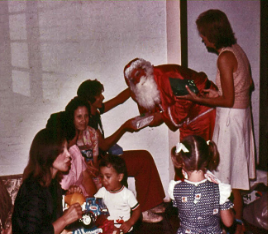
\includegraphics[width=0.6\linewidth]{28/distribuição.png}
\caption{Renatão distribuindo os presentes.}
\end{figure}


Quando acabava a distribuição dos brinquedos, a praxe era que a meninada fosse até a varanda dizer adeus a Papai Noel que, a bordo da carrocinha do sítio, toda enfeitada, sumia na escuridão da estrada sacudindo um sino em despedida.
Assim que ele desaparecia na curva, tratávamos de engambelar os pequenos tangendo-os rapidamente para o salão da ceia, para que o artista pudesse retornar à casa pulando a janela de um dos quartos e, livrando-se da fantasia e da maquilagem, aparecer na festa sem que Alessandra e Renata, as filhas, dessem pela sua ausência.
O ritual funcionou por muito tempo, até a noite em que, no afã de levar as crianças para o salão e dar-lhes de comer, esquecemos o Renatão lá fora, esmurrando desconsoladamente a janela, sem que ninguém o ouvisse naquela balbúrdia.
Passou-se bem uma hora antes que minha irmã notasse a falta do infeliz.

Numa outra vez em que tivemos que finalmente aposentar o Renato, pois as filhas já o adivinhavam pela voz e pelo jeito e tentavam, a todo custo, puxar-lhe a barba e a peruca, a brincadeira quase terminou em tragédia.
A escolhida para substituí-lo foi Tia Neta que, com seu rosto bonito, deu, segundo mamãe, o Papai Noel mais engraçadinho de todos e embatucou os meninos com seu mutismo.
Apesar da estranheza causada por este detalhe, a entrega de presentes foi um sucesso.
O problema se deu no momento da despedida.
Ao primeiro bimbalhar do sino, o burrico que puxava a carrocinha desembestou morro abaixo e as crianças, espantadíssimas, viram Noel virar de pernas para o ar e finalmente falar, mais do que isso, berrar, esgoelar por socorro em trinados de soprano lírico.

Quem mais se divertia com essa encenação toda era meu pai.
Na verdade, a excitação e o deslumbramento da meninada ao desembrulhar os brinquedos valiam a noite para ele.
Paulo e eu, com cinco filhos, nem pensávamos em comprar presentes caros.
A gente embrulhava um monte de coisas baratas de que toda criança gosta, carrinhos de plástico, cachimbo de fazer bolha de sabão, toquinhos coloridos de madeira, lápis de cor, livros de figura, quebra-cabeças, jogo de palitos e era aquela alegria.
Uma vez surpreendi meu pai abraçando carinhosamente Marcelo porque o moleque, no auge da felicidade ao ouvir seu nome chamado pela segunda ou terceira vez pelo Papai Noel, gritou para o avô, assanhadíssimo:

\textit{``-- Segure aí meus presentes, Vô, porque hoje eu tô com sorte. Ele tá me chamando de novo!''}

Isso, sem ligar minimamente para o fato de que os brinquedos que ganhara eram bem mais ordinários que os das primas.
Meu pai achou aquilo o máximo.

Marcou época no sítio o batizado do Marcelo.
Uma amiga minha, Sônia, casada com um colega do Paulo, quis batizar junto o filho deles.
Ocorre que na família dela havia um ilustre monsenhor, na bica para ser elevado a bispo, que foi convidado a realizar a cerimônia, fato que acendeu no vigário da nossa Matriz o desejo de acolitá-lo.
Zô, o marido da Sônia, por sua vez, tinha amigos no governo e alguns parentes ricos que não podia deixar de chamar para o evento.
Foi assim que, na data marcada, aportou sob a pérgula do estacionamento, um magote de gente importante, Monsenhor à frente, todo paramentado no rigor da liturgia, seguido bem de perto pelo baboso vigário e pela deslumbrada Vó Didi, que não tirava os olhos do anelão de Sua Excelência, à espera do momento oportuno para beijá-lo.
Na porta, uma Lectícia excitadíssima esperava a comitiva, ao lado do meu pai.

\begin{figure}
\centering
\includegraphics[width=0.6\linewidth]{28/casa-do-sítio.png}
\caption{A casa do sítio.}
\end{figure}

A casa do sítio, recém-inaugurada, obedeceu a todas as fantasias da minha mãe, que meu pai se divertira em realizar.
O estilo era colonial, tal como ela o entendia e explicava, mostrando os grandes lajotões de barro do piso, envelhecidos a poder de óleo queimado, as janelas em arco, pouco depois substituídas, e os ladrilhos estampados em rosáceas dos banheiros.
Ah, sim, e havia também os balaústres de madeira recortada da varanda.
Lá fora, o extenso gramado, a churrasqueira e as duas piscinas, para os adultos e para as crianças, completavam adequadamente aquilo que, para a filha de Didi e João, era uma casa de campo ``comme Il faut''.
Mamãe ficava muito orgulhosa de mostrar tudo às visitas e o ponto alto do roteiro era a enorme tesoura central sobre o salão que dividia as duas alas da casa e que tivera que ser reforçada para não vergar sob o peso do telhado.

À vista do cortejo e sentindo o clima que se anunciava, Renatão entrou em campo.
Abandonando a churrasqueira, deu um jeito de soprar ao ouvido da minha mãe: 

\textit{``-- Sônia me disse que o Monsenhor é louco por construções coloniais.''}

Era a deixa que ela esperava.
Um Renato torcido em riso ia antecipando baixinho para a gente tudo o que a mamãe diria em seguida ao atônito religioso, durante a minuciosa vistoria a que se viu arrastado e no decorrer da qual ouviu detalhadamente explicada a questão dos arcos, dos balaústres, dos lajotões escurecidos, dos ladrilhos em rosáceas, etc., etc., etc.
Finalmente, entre gargalhadas, meu cunhado chegou à apoteose, segundos antes que a anfitriã e o Monsenhor apontassem na porta do salão.
Erguendo-se delicadamente nas pontas dos pés e fazendo um gesto na direção da tesoura, declamou, imitando mamãe:

\textit{``-- E aqui está o que foi o nosso maior desafio.
Já viu uma tesoura assim? Mas eu não podia abrir mão da idéia de fazer um salão como esse, não acha? Afinal, numa ocasião como hoje, onde eu acomodaria tanta gente, não é mesmo?''}

E, cruzando as mãos com elegância:

\textit{``-- Então, o que o senhor achou? Tudo o que viu aqui foi pensado por mim.
Não pense que teve mão de arquiteto, não.
Gostou?''}

No momento em que mamãe estacionou Monsenhor e seus acompanhantes no meio do salão e ergueu teatralmente o braço na direção da tesoura, nem esperamos pelo resto.
Fomos rebentar de rir lá na beira da piscina.

Mas Renato não estava disposto a facilitar a vida da autoridade eclesiástica.
Mal a excelência abancou-se na sala para uma rápida conversa antes de dar início ao batizado, o gordo endemoninhado saiu à caça da Vó Didi e, assim que a encontrou, foi dizendo na maior aflição:

\textit{``-- Ô, Dona Didi, ainda bem que encontrei a senhora.
O Monsenhor me disse que não comeu durante a viagem, está morrendo de fraqueza, não sabe nem se aguenta fazer o batizado, mas está sem graça de pedir a comida antes dos outros.
Afinal, não conhece ninguém aqui.''}

Vovó nem pestanejou.
Ligeira, correu para a cozinha e avançando sobre as panelas, em segundos depôs diante do ilustre reverendo uma formidável marmita de pedreiro.
Nem que percorresse em jejum o Caminho de Santiago o coitado arranjaria apetite para encarar aquele despropósito de comida.
Pelo menos foi o que ele, balbuciante, tentou explicar à prestativa Didi, enquanto se levantava, tentando ir em direção à capela e alegando estar atrasado para a cerimônia.
Mas, vovó, lembrada do que Renato dissera sobre o constrangimento do santo homem em dar a conhecer sua fome, cortava-lhe o caminho e insistia para que comesse, fosse lá ele desmaiar no meio do batizado! A hilária sarabanda durou mais alguns segundos, com o Monsenhor tentando driblar a velhinha pela esquerda e pela direita até que, desesperado, fugiu para o banheiro, enquanto tratávamos de rebocar Didi e seu prato para fora de cena.


Inconformada, vovó teve que reduzir suas pretensões de alimentar um representante de Deus ao nosso vigário local que, aparentemente agradecido pela boa lembrança, devorou não só aquele, como todos os outros pratos que lhe foram oferecidos no decorrer do dia.
Alarmados com a vermelhidão que aos poucos lhe subia pelo pescoço e pela cara, alguns de nós já apostávamos numa explosão, imaginando seus sagrados intestinos pendurados feito liames nas árvores do pomar.
Ledo engano.
Passados mais de trinta anos, ele continua lá, beatificamente instalado na paróquia e na vida, desfrutando daquela disposição para a boa mesa que fez sua legenda na cidade.
 

\begin{figure}[H]
\hfill
\centering
\begin{subfigure}[h]{0.45\linewidth}
\centering
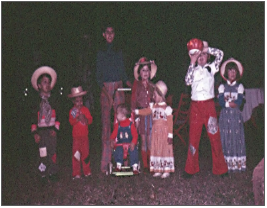
\includegraphics[width=\linewidth]{28/festa-junina.png}
\caption{Fantasiados para a festa junina.}
\end{subfigure}
\hfill
\begin{subfigure}[h]{0.45\linewidth}
\centering
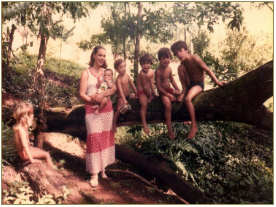
\includegraphics[width=1\linewidth]{28/com-os-cinco.png}
\caption{Com os cinco na véspera de Natal.}
\end{subfigure}
\end{figure}

\begin{figure}\ContinuedFloat
\hfill
\centering
\begin{subfigure}[h]{0.4\linewidth}
\centering
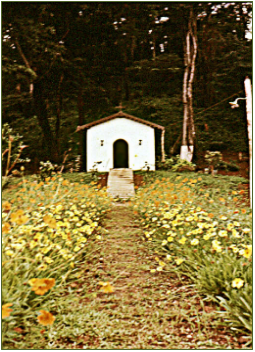
\includegraphics[width=\linewidth]{28/capela.png}
\caption{A capela do sítio.}
\end{subfigure}
\hfill
\begin{subfigure}[h]{0.4\linewidth}
\centering
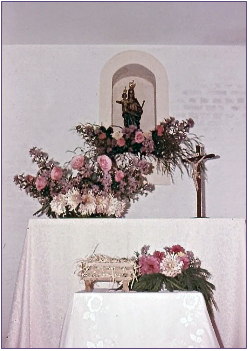
\includegraphics[width=1\linewidth]{28/altar-enfeitado.png}
\caption{O altar enfeitado para o Natal.}
\end{subfigure}
\end{figure}

\begin{figure}\ContinuedFloat
\hfill
\centering
\begin{subfigure}[h]{0.4\linewidth}
\centering
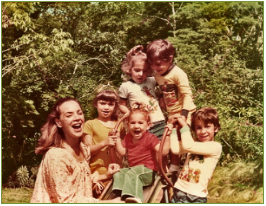
\includegraphics[width=\linewidth]{28/brincando.png}
\caption{Brincando no parquinho do sítio.}
\end{subfigure}
\hfill
\begin{subfigure}[h]{0.4\linewidth}
\centering
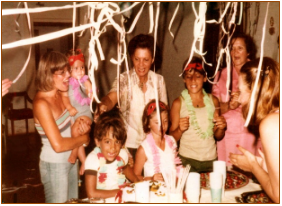
\includegraphics[width=1\linewidth]{28/niver-alessandra.png}
\caption{Aniversário da Alessandra.}
\end{subfigure}
\end{figure}

\begin{figure}\ContinuedFloat
\hfill
\centering
\begin{subfigure}[h]{0.4\linewidth}
\centering
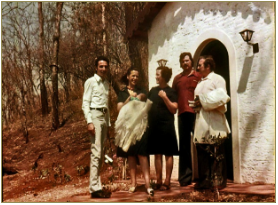
\includegraphics[width=\linewidth]{28/batizado-fernando.png}
\caption{O batizado do Fernando.}
\end{subfigure}
\hfill
\begin{subfigure}[h]{0.4\linewidth}
\centering
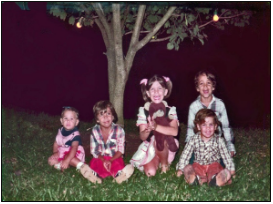
\includegraphics[width=1\linewidth]{28/esperando-ceia.png}
\caption{Esperando a ceia de Natal.}
\end{subfigure}
\end{figure}
